\documentclass{article}\usepackage{graphicx, color}
%% maxwidth is the original width if it is less than linewidth
%% otherwise use linewidth (to make sure the graphics do not exceed the margin)
\makeatletter
\def\maxwidth{ %
  \ifdim\Gin@nat@width>\linewidth
    \linewidth
  \else
    \Gin@nat@width
  \fi
}
\makeatother

\definecolor{fgcolor}{rgb}{0.2, 0.2, 0.2}
\newcommand{\hlnumber}[1]{\textcolor[rgb]{0,0,0}{#1}}%
\newcommand{\hlfunctioncall}[1]{\textcolor[rgb]{0.501960784313725,0,0.329411764705882}{\textbf{#1}}}%
\newcommand{\hlstring}[1]{\textcolor[rgb]{0.6,0.6,1}{#1}}%
\newcommand{\hlkeyword}[1]{\textcolor[rgb]{0,0,0}{\textbf{#1}}}%
\newcommand{\hlargument}[1]{\textcolor[rgb]{0.690196078431373,0.250980392156863,0.0196078431372549}{#1}}%
\newcommand{\hlcomment}[1]{\textcolor[rgb]{0.180392156862745,0.6,0.341176470588235}{#1}}%
\newcommand{\hlroxygencomment}[1]{\textcolor[rgb]{0.43921568627451,0.47843137254902,0.701960784313725}{#1}}%
\newcommand{\hlformalargs}[1]{\textcolor[rgb]{0.690196078431373,0.250980392156863,0.0196078431372549}{#1}}%
\newcommand{\hleqformalargs}[1]{\textcolor[rgb]{0.690196078431373,0.250980392156863,0.0196078431372549}{#1}}%
\newcommand{\hlassignement}[1]{\textcolor[rgb]{0,0,0}{\textbf{#1}}}%
\newcommand{\hlpackage}[1]{\textcolor[rgb]{0.588235294117647,0.709803921568627,0.145098039215686}{#1}}%
\newcommand{\hlslot}[1]{\textit{#1}}%
\newcommand{\hlsymbol}[1]{\textcolor[rgb]{0,0,0}{#1}}%
\newcommand{\hlprompt}[1]{\textcolor[rgb]{0.2,0.2,0.2}{#1}}%

\usepackage{framed}
\makeatletter
\newenvironment{kframe}{%
 \def\at@end@of@kframe{}%
 \ifinner\ifhmode%
  \def\at@end@of@kframe{\end{minipage}}%
  \begin{minipage}{\columnwidth}%
 \fi\fi%
 \def\FrameCommand##1{\hskip\@totalleftmargin \hskip-\fboxsep
 \colorbox{shadecolor}{##1}\hskip-\fboxsep
     % There is no \\@totalrightmargin, so:
     \hskip-\linewidth \hskip-\@totalleftmargin \hskip\columnwidth}%
 \MakeFramed {\advance\hsize-\width
   \@totalleftmargin\z@ \linewidth\hsize
   \@setminipage}}%
 {\par\unskip\endMakeFramed%
 \at@end@of@kframe}
\makeatother

\definecolor{shadecolor}{rgb}{.97, .97, .97}
\definecolor{messagecolor}{rgb}{0, 0, 0}
\definecolor{warningcolor}{rgb}{1, 0, 1}
\definecolor{errorcolor}{rgb}{1, 0, 0}
\newenvironment{knitrout}{}{} % an empty environment to be redefined in TeX

\usepackage{alltt}
\usepackage{amsmath}
\IfFileExists{upquote.sty}{\usepackage{upquote}}{}
\begin{document}
\title{London R Practice}
\author{Rob Hayward}
\maketitle
\section{Introduction}

This is a file to run through the presentation that was made at the September 2013 London R by Maarten Speekenbrink.  

I am not sure how to load the appropriate packages (so this can probably be deleted in the future).  However, I will do that in a chunk. The information is in the title:  dependent mixed models. This is to implement micture and hidden Markov models. 


\section{Mixed Models}
From the London R presentation. In a \emph{mixture model} each observation is assumed to be drawn from a number of distinct subpopulation (``component distributions'' according to Maarten).  The distribution from which the observation is drawn is not directly observable and therefore it is represented by a \emph{latent state}.  

A mixture distribution is defined as 
\begin{equation}
p(Y_1 = y) = \sum_{i - 1}^N p(Y_t = y|S_t = i)P(S_t = i)
\end{equation}
where,
\begin{itemize}
\item $S_t \in {1, \dots, N}$ denotes the latent state or class of observation t
\item $P(S_t = i)$ denots the probability of the latent state t equals i 
\item $p(Y_t = y|S_t = i)$ denotes the density of observation of $Y_t$ conditional on latent state being $S_t = i$.
\end{itemize}
\section{Perth Water Example}

First download the data and plot. 
\begin{knitrout}
\definecolor{shadecolor}{rgb}{0.969, 0.969, 0.969}\color{fgcolor}\begin{kframe}
\begin{alltt}
da <- \hlfunctioncall{read.csv}(\hlstring{"./Perth.csv"}, header = TRUE)
\hlfunctioncall{plot}(da$water, type = \hlstring{"l"}, main = \hlstring{"Perth Dams Water flow"})
\end{alltt}
\end{kframe}
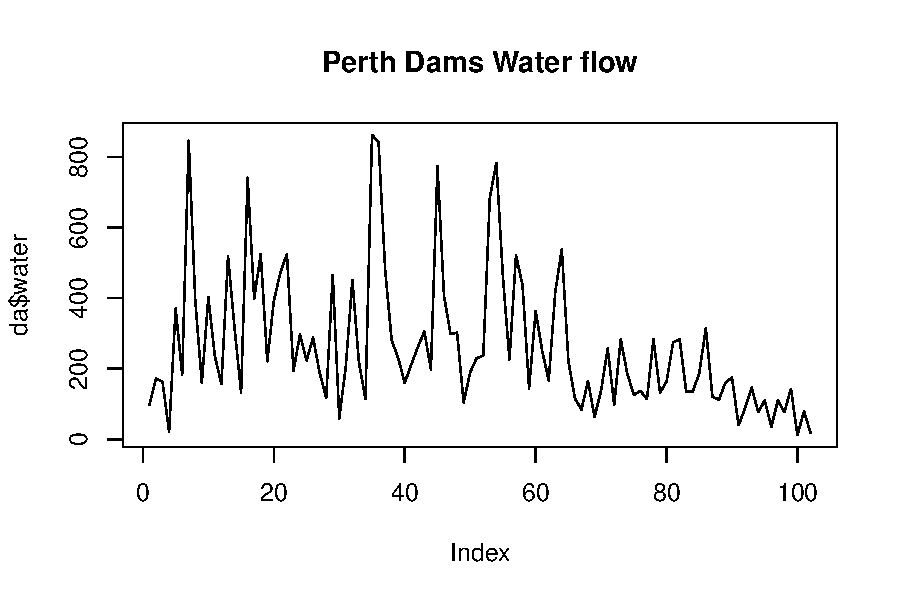
\includegraphics[width=\maxwidth]{figure/perth} 

\end{knitrout}

The aim is to model the water flow. the typical method would try to impose a level model (lm1) or a linear (lmyr) or quadratic model (lmyr2).
\begin{kframe}
\begin{alltt}
lm1 <- \hlfunctioncall{lm}(da$water ~ 1, data = da)
lmyr <- \hlfunctioncall{lm}(da$water ~ yr, data = da)
lmyr2 <- \hlfunctioncall{lm}(da$water ~ yr + \hlfunctioncall{I}(yr^2), data = da)
dd <- \hlfunctioncall{xtable}(\hlfunctioncall{anova}(lm1, lmyr, lmyr2), digits = 2)
\hlfunctioncall{print}(dd)
\end{alltt}
\end{kframe}% latex table generated in R 2.15.2 by xtable 1.7-0 package
% Sun Sep 22 21:42:52 2013
\begin{table}[ht]
\begin{center}
\begin{tabular}{lrrrrrr}
  \hline
 & Res.Df & RSS & Df & Sum of Sq & F & Pr($>$F) \\ 
  \hline
1 & 101.00 & 3811695.17 &  &  &  &  \\ 
  2 & 100.00 & 3257024.21 & 1.00 & 554670.95 & 18.68 & 0.00 \\ 
  3 & 99.00 & 2939677.35 & 1.00 & 317346.87 & 10.69 & 0.00 \\ 
   \hline
\end{tabular}
\end{center}
\end{table}


The linear and quadratic equiations show a vaiance that is significantly lower than the model with just the fixed level. 
\begin{knitrout}
\definecolor{shadecolor}{rgb}{0.969, 0.969, 0.969}\color{fgcolor}\begin{kframe}
\begin{alltt}
da <- \hlfunctioncall{read.csv}(\hlstring{"./Perth.csv"}, header = TRUE)
\hlfunctioncall{plot}(da$water, type = \hlstring{"l"}, main = \hlstring{"Fitted Perth Dams Water flow"})
\hlfunctioncall{lines}(lm1$fitted, col = \hlstring{"dark green"})
\hlfunctioncall{lines}(lmyr$fitted, col = \hlstring{"blue"})
\hlfunctioncall{lines}(lmyr2$fitted, col = \hlstring{"red"})
\hlfunctioncall{legend}(x = 80, y = 650, legend = \hlfunctioncall{c}(\hlstring{"lm1"}, \hlstring{"lmyr"}, \hlstring{"lmyr2"}))
\end{alltt}
\end{kframe}
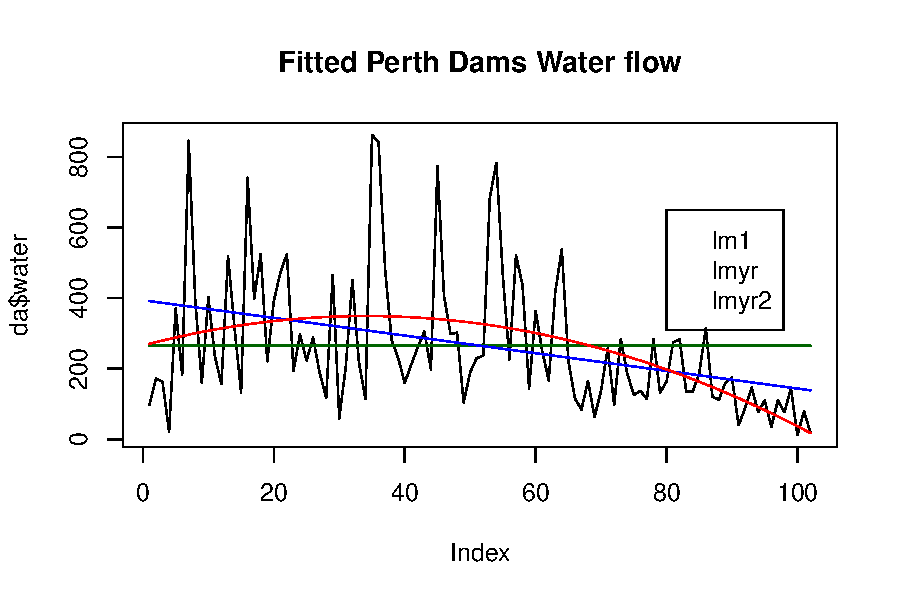
\includegraphics[width=\maxwidth]{figure/perth2} 

\end{knitrout}

AR models can also be used and assessed using the Akaike Information Criteria or Bayesian Information Criteria. 
\begin{knitrout}
\definecolor{shadecolor}{rgb}{0.969, 0.969, 0.969}\color{fgcolor}\begin{kframe}
\begin{alltt}
arOrder <- \hlfunctioncall{ar}(da$water)$order
ar1 <- \hlfunctioncall{arima}(da$water, \hlfunctioncall{c}(arOrder, 0, 0))
aryr <- \hlfunctioncall{arima}(da$water, \hlfunctioncall{c}(arOrder, 0, 0), xreg = da$yr)
aryr2 <- \hlfunctioncall{arima}(da$water, \hlfunctioncall{c}(arOrder, 0, 0), xreg = \hlfunctioncall{cbind}(yr = \hlfunctioncall{scale}(da$yr), yr2 = \hlfunctioncall{scale}(da$yr)^2))
\hlfunctioncall{print}(\hlfunctioncall{c}(ar1 = \hlfunctioncall{AIC}(ar1), aryr = \hlfunctioncall{AIC}(aryr), aryr2 = \hlfunctioncall{AIC}(aryr2)))
\end{alltt}
\begin{verbatim}
##   ar1  aryr aryr2 
##  1355  1349  1344
\end{verbatim}
\begin{alltt}
\hlfunctioncall{print}(\hlfunctioncall{c}(lm1 = \hlfunctioncall{AIC}(lm1), lmyr = \hlfunctioncall{AIC}(lmyr), lmyr2 = \hlfunctioncall{AIC}(lmyr2)))
\end{alltt}
\begin{verbatim}
##   lm1  lmyr lmyr2 
##  1367  1353  1345
\end{verbatim}
\end{kframe}
\end{knitrout}


\begin{knitrout}
\definecolor{shadecolor}{rgb}{0.969, 0.969, 0.969}\color{fgcolor}\begin{kframe}
\begin{alltt}
\hlfunctioncall{require}(forecast)
da <- \hlfunctioncall{read.csv}(\hlstring{"./Perth.csv"}, header = TRUE)
\hlfunctioncall{plot}(da$water, type = \hlstring{"l"}, main = \hlstring{"AR Fitted Perth Dams Water flow"})
\hlfunctioncall{lines}(\hlfunctioncall{fitted}(aryr), col = \hlstring{"dark green"})
\hlfunctioncall{lines}(\hlfunctioncall{fitted}(aryr2), col = \hlstring{"blue"})
\hlfunctioncall{lines}(\hlfunctioncall{fitted}(ar1), col = \hlstring{"red"})
\hlfunctioncall{legend}(x = 80, y = 650, legend = \hlfunctioncall{c}(\hlstring{"ar1"}, \hlstring{"aryr"}, \hlstring{"aryr2"}))
\end{alltt}
\end{kframe}
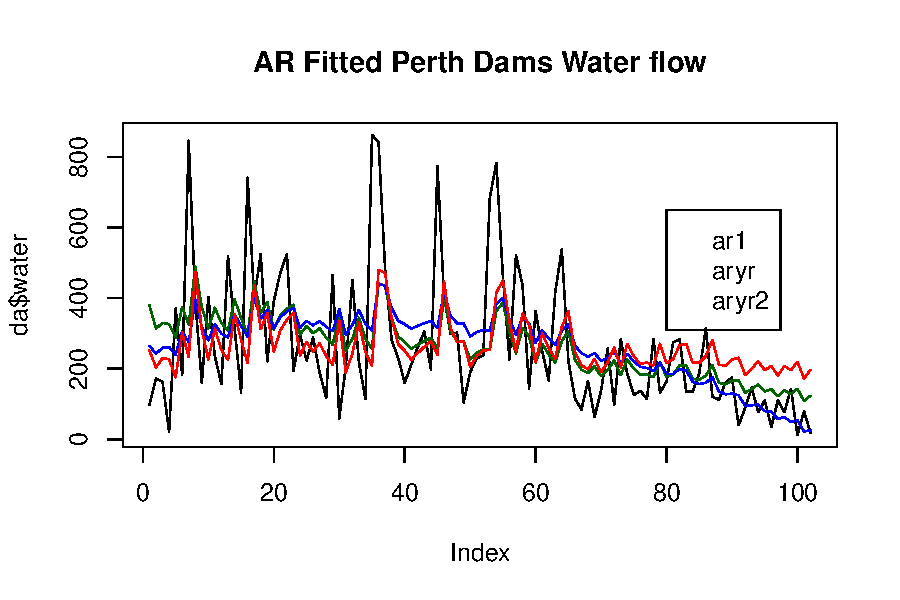
\includegraphics[width=\maxwidth]{figure/perth3} 

\end{knitrout}



\section{Change Model}
This is a model that assumes one or more discrete change points in the data. It may be the mean, trend or other parameters that may change. In this example with the S\&P 500 it is the mean and the standard deviation. There is a transition matrix that defines the change points.  For example, if there is one transition the matrix would be along the lines of 
\begin{equation*}
\begin{pmatrix}
p_1 & 1 - p_1 \\
0 & 1
\end{pmatrix}
\end{equation*}
Where $p_1$ is the probability that the system will be in state 1.  One there is a switch to state two.  This matrix can be extended for more states. Need to come back and look at this if I can get the data. 
\begin{knitrout}
\definecolor{shadecolor}{rgb}{0.969, 0.969, 0.969}\color{fgcolor}\begin{kframe}
\begin{alltt}
mod2 <- \hlfunctioncall{depmix}(water ~ 1, data = da, ns = 2, trst = \hlfunctioncall{c}(0.9, 0.1, 0, 1), inst = \hlfunctioncall{c}(1, 
    0))
\hlfunctioncall{set.seed}(1)
fm2 <- \hlfunctioncall{fit}(mod2, verbose = FALSE)
\end{alltt}
\begin{verbatim}
## iteration 3 logLik: -654.5
\end{verbatim}
\begin{alltt}
\hlfunctioncall{summary}(fm2)
\end{alltt}
\begin{verbatim}
## Initial state probabilties model 
## Model of type multinomial (identity), formula: ~1
## <environment: 0x0000000008b89cd0>
## Coefficients: 
##      [,1] [,2]
## [1,]    1    0
## 
## Transition model for state (component) 1 
## Model of type multinomial (identity), formula: ~1
## <environment: 0x000000000867dd80>
## Coefficients: 
## [1] 0.9845 0.0155
## 
## Transition model for state (component) 2 
## Model of type multinomial (identity), formula: ~1
## <environment: 0x000000000867dd80>
## Coefficients: 
## [1] 0 1
## 
## 
## Response model(s) for state 1 
## 
## Response model for response 1 
## Model of type gaussian (identity), formula: water ~ 1
## Coefficients: 
## [1] 337
## sd  204.1 
## 
## 
## Response model(s) for state 2 
## 
## Response model for response 1 
## Model of type gaussian (identity), formula: water ~ 1
## Coefficients: 
## [1] 141.4
## sd  76.16
\end{verbatim}
\end{kframe}
\end{knitrout}

The information here is the inital state probabilities, the transition model for state 1 and state 2; the response model for state 1 and the response model for state 2.  These show a mean value of 337 and 141 respectively and a standard deviation of 204.1 and 76.16.  There is a decline in the amount of water and there is a fall in the variability. 

The posterior() function can be used to obtain the maximum \emph{a posteriori} state sequence (column 1) and the posterior state probabilities (remaining columns).  
\begin{knitrout}
\definecolor{shadecolor}{rgb}{0.969, 0.969, 0.969}\color{fgcolor}\begin{kframe}
\begin{alltt}
pst <- \hlfunctioncall{posterior}(fm2)
\hlfunctioncall{head}(pst)
\end{alltt}
\begin{verbatim}
##   state     X1      X2
## 1     1 1.0000 0.00000
## 2     1 0.9489 0.05110
## 3     1 0.8312 0.16875
## 4     1 0.6558 0.34420
## 5     1 0.9849 0.01513
## 6     1 0.9536 0.04642
\end{verbatim}
\begin{alltt}
\hlfunctioncall{tail}(pst)
\end{alltt}
\begin{verbatim}
##     state        X1 X2
## 97      2 3.266e-13  1
## 98      2 7.622e-14  1
## 99      2 1.783e-14  1
## 100     2 7.811e-15  1
## 101     2 1.806e-15  1
## 102     2 7.272e-16  1
\end{verbatim}
\begin{alltt}
pst[, 1]
\end{alltt}
\begin{verbatim}
##   [1] 1 1 1 1 1 1 1 1 1 1 1 1 1 1 1 1 1 1 1 1 1 1 1 1 1 1 1 1 1 1 1 1 1 1 1
##  [36] 1 1 1 1 1 1 1 1 1 1 1 1 1 1 1 1 1 1 1 1 1 1 1 1 1 1 1 1 1 2 2 2 2 2 2
##  [71] 2 2 2 2 2 2 2 2 2 2 2 2 2 2 2 2 2 2 2 2 2 2 2 2 2 2 2 2 2 2 2 2
\end{verbatim}
\end{kframe}
\end{knitrout}

\section{S\&P 500 Example}
\begin{knitrout}
\definecolor{shadecolor}{rgb}{0.969, 0.969, 0.969}\color{fgcolor}\begin{kframe}
\begin{alltt}
\hlfunctioncall{library}(TTR)
\hlcomment{# load SP500 returns}
\hlfunctioncall{Sys.setenv}(tz = \hlstring{"UTC"})
sp500 <- \hlfunctioncall{getYahooData}(\hlstring{"^GSPC"}, start = 19500101, end = 20120909, freq = \hlstring{"daily"})
ep <- \hlfunctioncall{endpoints}(sp500, on = \hlstring{"months"}, k = 1)
sp500 <- sp500[ep[2:(\hlfunctioncall{length}(ep) - 1)]]
sp500$logret <- \hlfunctioncall{log}(sp500$Close) - \hlfunctioncall{lag}(\hlfunctioncall{log}(sp500$Close))
sp500 <- \hlfunctioncall{na.exclude}(sp500)
\end{alltt}
\end{kframe}
\end{knitrout}

Now plot the data to get an idea of what it looks like. 
\begin{knitrout}
\definecolor{shadecolor}{rgb}{0.969, 0.969, 0.969}\color{fgcolor}\begin{kframe}
\begin{alltt}
\hlfunctioncall{plot}(sp500$logret, main = \hlstring{"S&P 500 log returns"})
\end{alltt}
\end{kframe}
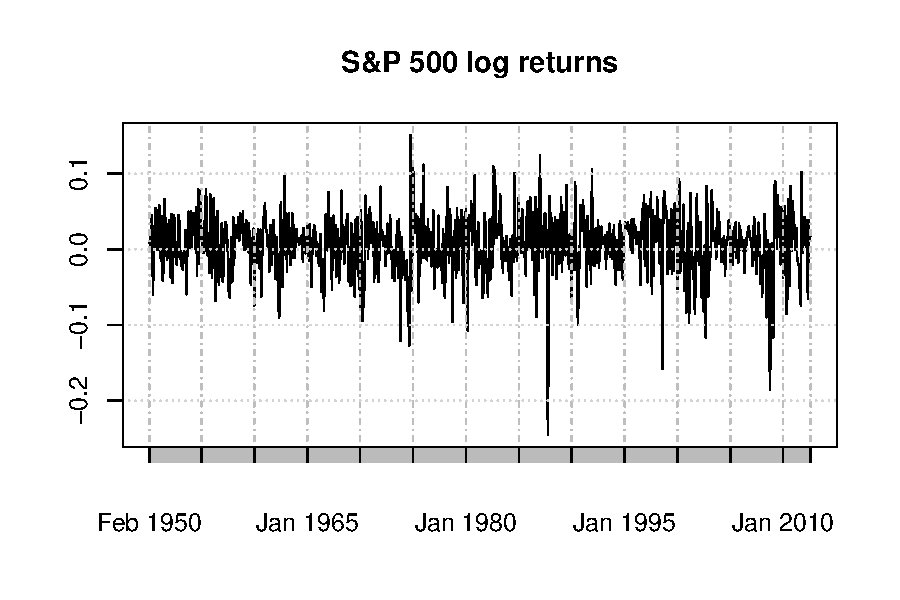
\includegraphics[width=\maxwidth]{figure/plot2} 

\end{knitrout}

The aim is to identify the bull and bear markets. First set up the model (mod). This is a model of the log return with two states. Then fit the model.   
\begin{knitrout}
\definecolor{shadecolor}{rgb}{0.969, 0.969, 0.969}\color{fgcolor}\begin{kframe}
\begin{alltt}
mod <- \hlfunctioncall{depmix}(logret ~ 1, nstates = 2, data = sp500)
\hlfunctioncall{set.seed}(1)
fm2 <- \hlfunctioncall{fit}(mod, verbose = FALSE)
\end{alltt}
\begin{verbatim}
## iteration 88 logLik: 1348
\end{verbatim}
\end{kframe}
\end{knitrout}

The number of iterations and the log likelihood is printed.  Now summarise the information. 
\begin{knitrout}
\definecolor{shadecolor}{rgb}{0.969, 0.969, 0.969}\color{fgcolor}\begin{kframe}
\begin{alltt}
depmixS4::\hlfunctioncall{summary}(fm2)
\end{alltt}
\begin{verbatim}
## Initial state probabilties model 
## Model of type multinomial (identity), formula: ~1
## <environment: 0x0000000008efd2c8>
## Coefficients: 
##           [,1] [,2]
## [1,] 1.735e-47    1
## 
## Transition model for state (component) 1 
## Model of type multinomial (identity), formula: ~1
## <environment: 0x0000000011cdddc0>
## Coefficients: 
## [1] 0.8215 0.1785
## 
## Transition model for state (component) 2 
## Model of type multinomial (identity), formula: ~1
## <environment: 0x0000000011cdddc0>
## Coefficients: 
## [1] 0.03914 0.96086
## 
## 
## Response model(s) for state 1 
## 
## Response model for response 1 
## Model of type gaussian (identity), formula: logret ~ 1
## Coefficients: 
## [1] -0.01505
## sd  0.06484 
## 
## 
## Response model(s) for state 2 
## 
## Response model for response 1 
## Model of type gaussian (identity), formula: logret ~ 1
## Coefficients: 
## [1] 0.01045
## sd  0.03378
\end{verbatim}
\end{kframe}
\end{knitrout}



\end{document}
